%%%%%%%%%%%%%%%%%%%%%%%%%%%%%%%%%%%%%%%%%%%%%%%%%%%%%%%%%%%%%%%%%%%%%%
% LaTeX Template: Project Titlepage
%
% Source: http://www.howtotex.com
% Date: April 2011
% 
% This is a title page template which be used for articles & reports.
% 
% Feel free to distribute this example, but please keep the referral
% to howtotex.com
% 
%%%%%%%%%%%%%%%%%%%%%%%%%%%%%%%%%%%%%%%%%%%%%%%%%%%%%%%%%%%%%%%%%%%%%%
% How to use writeLaTeX: 
%
% You edit the source code here on the left, and the preview on the
% right shows you the result within a few seconds.
%
% Bookmark this page and share the URL with your co-authors. They can
% edit at the same time!
%
% You can upload figures, bibliographies, custom classes and
% styles using the files menu.
%
% If you're new to LaTeX, the wikibook is a great place to start:
% http://en.wikibooks.org/wiki/LaTeX
%
%%%%%%%%%%%%%%%%%%%%%%%%%%%%%%%%%%%%%%%%%%%%%%%%%%%%%%%%%%%%%%%%%%%%%%
%
% --------------------------------------------------------------------
% Preamble
% --------------------------------------------------------------------
\documentclass[paper=a4, fontsize=11pt,twoside]{scrartcl}	% KOMA

\usepackage[a4paper,pdftex]{geometry}	% A4paper margins
\setlength{\oddsidemargin}{5mm}			% Remove 'twosided' indentation
\setlength{\evensidemargin}{5mm}

\usepackage[english]{babel}
\usepackage[protrusion=true,expansion=true]{microtype}	
\usepackage{amsmath,amsfonts,amsthm,amssymb}
\usepackage{graphicx}
\usepackage{float}
% --------------------------------------------------------------------
% Definitions (do not change this)
% --------------------------------------------------------------------
\newcommand{\HRule}[1]{\rule{\linewidth}{#1}} 	% Horizontal rule

\makeatletter							% Title
\def\printtitle{%						
    {\centering \@title\par}}
\makeatother									

\makeatletter							% Author
\def\printauthor{%					
    {\centering \large \@author}}				
\makeatother							

% --------------------------------------------------------------------
% Metadata (Change this)
% --------------------------------------------------------------------
\title{	\normalsize \textsc{Project Report} 	% Subtitle
		 	\\[2.0cm]								% 2cm spacing
			\HRule{0.5pt} \\						% Upper rule
			\LARGE \textbf{\uppercase{Sample Sizes for Query Probing in Distributed Information Retreival}}	% Title
			\HRule{2pt} \\ [0.5cm]		% Lower rule + 0.5cm spacing
			\normalsize \today			% Todays date
		}

\author{
		Rahul Ramakrishna\\	
		University of Massachussets Amherst\\	
		Dept Of Computer Science\\
        \texttt{rahulram@cs.umass.edu} \\
}


\begin{document}
% ------------------------------------------------------------------------------
% Maketitle
% ------------------------------------------------------------------------------
\thispagestyle{empty}		% Remove page numbering on this page

\printtitle					% Print the title data as defined above
  	\vfill
\printauthor				% Print the author data as defined above
\newpage
% ------------------------------------------------------------------------------
% Begin document
% ------------------------------------------------------------------------------
\setcounter{page}{1}		% Set page numbering to begin on this page
\section{Introduction}

In Distributed Information Reterival systems, information is held in separate collections, which might be in different physical locations or on separate servers. The query is first passed to a central
broker. The broker then sends this query to all or some of the servers. The cost of networking during query execution seems an overhead, escepially if the query is sent to servers which dont have similar collections.

\begin{figure}[H]
\centering
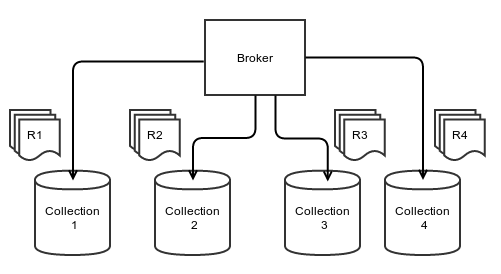
\includegraphics[width=\textwidth]{./img/ir.png}
\caption{\label{fig:1}DIR System.}
\end{figure}


Thus, DIR has 2 major issues to be resolved. 
\begin{enumerate}
\item Selection of a particular collection
\item Merging of Results.
\end{enumerate}
In this report, we are mainly focusing on selection of collections. We are focusing on how to characterize a 
particular collection such that, the broker can decide on which servers to send the queries to further probe for 
results. We further explore 2 main sampling techniques which are used to represent collection of sets.


\section{Sampling Techniques}
\label{sec:examples}




\subsection{Query Probing}
In non-cooperative environments like distributed systems. We dont get index information from each of the collections that are being fetched. Instead, its the brokers that constantly probe into the collection by sending artificial queries in random order and evaluate returned answers. The answers are called \texttt{probes} 
and the process is called \texttt{query probing}. For example, if we send a series of single probe queries such as "books", "football", "ibm" and the following number of answers are returned: 1000, 200, 450 .


\subsection{Static Sampling using Ctf}

Use \texttt{section}s and \texttt{subsection}s to organize your document. \LaTeX{} handles all the formatting and numbering automatically. Use \texttt{ref} and \texttt{label} for cross-references --- this is Section~\ref{sec:examples}, for example.



\subsection{Adaptive Query Probing}

Use \texttt{tabular} for basic tables. You can upload a figure (JPEG, PNG or PDF) using the files menu. To include it in your document, use the \texttt{includegraphics} command (see the comment below in the source code).

% Commands to include a figure:
%\begin{figure}
%\includegraphics[width=\textwidth]{your-figure's-file-name}
%\caption{\label{fig:your-figure}Caption goes here.}
%\end{figure}

\subsection{Mathematics}

\LaTeX{} is great at typesetting mathematics. Let $X_1, X_2, \ldots, X_n$ be a sequence of independent and identically distributed random variables with $\text{E}[X_i] = \mu$ and $\text{Var}[X_i] = \sigma^2 < \infty$, and let
$$S_n = \frac{X_1 + X_2 + \cdots + X_n}{n}
      = \frac{1}{n}\sum_{i}^{n} X_i$$
denote their mean. Then as $n$ approaches infinity, the random variables $\sqrt{n}(S_n - \mu)$ converge in distribution to a normal $\mathcal{N}(0, \sigma^2)$.

\section{Measure of Effectiveness}

You can make lists with automatic numbering \dots

\dots or bullet points \dots
\begin{itemize}
\item Like this,
\item and like this.
\end{itemize}




% ------------------------------------------------------------------------------
% End document
% ------------------------------------------------------------------------------
\end{document}
